\section{Xây dựng cây cú pháp trừu tượng}

\textbf{NOTE:} Nhắc đến việc sử dụng thư viện Syn, Rust chưa có đặc tả chính thức mà có reference. Thư viện syn có ngữ pháp tuân theo reference này. Tất cả các loại AST sẽ tuân theo định nghĩa của thư viện Syn.

\begin{figure}[H]
	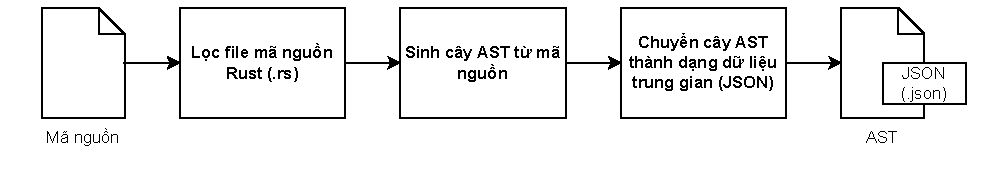
\includegraphics[width=1\columnwidth]{figures/c3/c3_flow_ast.drawio.pdf}
	\centering
	\caption{Quy trình xây dựng cây cú pháp trừu tượng}
	\label{img:method_flow_ast}
\end{figure}

Quy trình xây dựng cây cú pháp trừu tượng bao gồm ba bước được thể hiện trong
Hình 3.2, chi tiết các bước được tiến hành như sau:

\begin{enumerate}
  \item Từ thư mục của dự án, lọc lấy các tệp mã nguồn Rust (các tệp có đuôi là .rs)
  \item Với mỗi tệp mã nguồn, sử dụng thư viện syn để phân tích thành cây cú pháp trừu tượng (AST) ứng với tệp đó.
  \item Chuyển đổi cây cú phá p trừu tượng thu được sang dạng cây tự định nghĩa. Về bản chất dạng cây tự định nghĩa này hoàn toàn giống với dạng cây gốc, tuy nhiên cây chỉ lưu các thông tin cần thiết cũng như bổ sung thêm một số thông tin để xác định nút cha, chữ ký nút và một số thông tin khác để phục vụ pha phân tích tiếp theo.
\end{enumerate}

Trong quá trình xây dựng cây cú pháp trừu tượng, các thành phần mã nguồn trong
Rust sẽ được phân tích thành dạng cây tương ứng. Dưới đây là một số hình ảnh ví dụ về
cây cú pháp trừu tượng ứng với các thành phần mã nguồn này.

Hình 3.3 biểu diễn một hàm được phân tích thành một nút định nghĩa hàm (Func-
tionDeclaration), nút này có các thuộc tính là chữ ký (signature), kiểu trả về (returnType)
và tên đầy đủ (fullName). Nút có các nút con gồm nút định danh (Identifier) biểu diễn
định danh của hàm, nút kiểu hàm (FunctionType) biểu diễn kiểu dữ liệu của hàm và nút
thân hàm (BlockStatement).

Ví dụ về biểu diễn một kiểu cấu trúc được thể hiện trong Hình 3.4. Nút TypeSpeci-
fication đại diện cho định nghĩa kiểu. Nút Identifier là nút định danh biểu diễn tên kiểu.
Nút StructType biểu diễn kiểu cấu trúc. Nút FieldList có các nút con là Field biểu diễn các thuộc tính của kiểu này.

\footnotesize
\begin{longtable}{| p{.07\textwidth} | p{.30\textwidth} | p{.63\textwidth} |}
\hline
\textbf{STT} & \textbf{Tên nút} & \textbf{Mô tả} \\ \hline
1     & Abi                            & The binary interface of a function: `extern "C"`.                                                              \\ \hline
2     & \makecell{AngleBracketed \\ GenericArguments} & Angle bracketed arguments of a path segment: the `<K, V>` in HashMap<K, V>.                                    \\ \hline
3     & Arm                            & One arm of a `match` expression: `0..=10 => { return true; }`.                                                 \\ \hline
4     & AssocConst                     & An equality constraint on an associated constant: `the PANIC = false in Trait<PANIC = false>`.                 \\ \hline
5     & AssocType                      & A binding (equality constraint) on an associated type: `the Item = u8 in Iterator<Item = u8>`.                 \\ \hline
6     & Attribute                      & An attribute, like `\#[repr(transparent)]`.                                                                     \\ \hline
7     & BareFnArg                      & An argument in a function type: `the usize in fn(usize) -> bool`.                                              \\ \hline
8     & BareVariadic                   & The variadic argument of a function pointer like `fn(usize, ...)`.                                             \\ \hline
9     & Block                          & A braced block containing Rust statements.                                                                     \\ \hline
10    & BoundLifetimes                 & A set of bound lifetimes: `for<'a, 'b, 'c>`.                                                                   \\ \hline
11    & ConstParam                     & A const generic parameter: `const LENGTH: usize`.                                                              \\ \hline
12    & Constraint                     & An associated type bound: `Iterator<Item: Display>`.                                                           \\ \hline
13    & DataEnum                       & An enum input to a `proc\_macro\_derive` macro.                                                                  \\ \hline
14    & DataStruct                     & A struct input to a `proc\_macro\_derive` macro.                                                                 \\ \hline
15    & DataUnion                      & An untagged union input to a `proc\_macro\_derive` macro.                                                        \\ \hline
16    & DeriveInput                    & Data structure sent to a `proc\_macro\_derive` macro.                                                            \\ \hline
17    & Error                          & Error returned when a Syn parser cannot parse the input tokens.                                                \\ \hline
18    & ExprArray                      & A slice literal expression: `[a, b, c, d]`.                                                                    \\ \hline
19    & ExprAssign                     & An assignment expression: `a = compute()`.                                                                     \\ \hline
20    & ExprAsync                      & An async block: `async { ... }`.                                                                               \\ \hline
21    & ExprAwait                      & An await expression: `fut.await`.                                                                              \\ \hline
22    & ExprBinary                     & A binary operation: `a + b, a += b`.                                                                           \\ \hline
23    & ExprBlock                      & A blocked scope: `{ ... }`.                                                                                    \\ \hline
24    & ExprBreak                      & A `break`, with an optional label to break and an optional expression.                                         \\ \hline
25    & ExprCall                       & A function call expression: `invoke(a, b)`.                                                                    \\ \hline
26    & ExprCast                       & A cast expression: `foo as f64`.                                                                               \\ \hline
27    & ExprClosure                    & A closure expression: `[a, b] + a + b`.                                                                        \\ \hline
28    & ExprConst                      & A const block: `const { ... }`.                                                                                \\ \hline
29    & ExprContinue                   & A `continue`, with an optional label.                                                                          \\ \hline
30    & ExprField                      & Access of a named struct field `obj.k` or unnamed tuple struct field `obj.0`.                                  \\ \hline
31    & ExprForLoop                    & A for loop: `for pat in expr { ... }`.                                                                         \\ \hline
32    & ExprGroup                      & An expression contained within invisible delimiters.                                                           \\ \hline
33    & ExprIf                         & An if expression with an optional else block: if expr { ... } else { ... }.                                    \\ \hline
34    & ExprIndex                      & A square bracketed indexing expression: vector[2].                                                             \\ \hline
35    & ExprInfer                      & The inferred value of a const generic argument, denoted \_.                                                    \\ \hline
36    & ExprLet                        & A let guard: let Some(x) = opt.                                                                                \\ \hline
37    & ExprLit                        & A literal in place of an expression: 1, "foo".                                                                 \\ \hline
38    & ExprLoop                       & Conditionless loop: loop { ... }.                                                                              \\ \hline
39    & ExprMacro                      & A macro invocation expression: format!("{}", q).                                                               \\ \hline
40    & ExprMatch                      & A match expression: match n { Some(n) => {}, None => {} }.                                                     \\ \hline
41    & ExprMethodCall                 & A method call expression: x.foo::<T>(a, b).                                                                    \\ \hline
42    & ExprParen                      & A parenthesized expression: (a + b).                                                                           \\ \hline
43    & ExprPath                       & A path like std::mem::replace possibly containing generic parameters and a qualified self-type.                \\ \hline
44    & ExprRange                      & A range expression: 1..2, 1.., ..2, 1..=2, ..=2.                                                               \\ \hline
45    & ExprRawAddr                    & Address-of operation: \&raw const place or \&raw mut place.                                                      \\ \hline
46    & ExprReference                  & A referencing operation: \&a or \&mut a.                                                                         \\ \hline
47    & ExprRepeat                     & An array literal constructed from one repeated element: [0u8; N].                                              \\ \hline
48    & ExprReturn                     & A return, with an optional value to be returned.                                                               \\ \hline
49    & ExprStruct                     & A struct literal expression: Point { x: 1, y: 1 }.                                                             \\ \hline
50    & ExprTry                        & A try-expression: expr?.                                                                                       \\ \hline
51    & ExprTryBlock                   & A try block: try { ... }.                                                                                      \\ \hline
52    & ExprTuple                      & A tuple expression: (a, b, c, d).                                                                              \\ \hline
53    & ExprUnary                      & A unary operation: !x, \*x.                                                                                    \\ \hline
54    & ExprUnsafe                     & An unsafe block: unsafe { ... }.                                                                               \\ \hline
55    & ExprWhile                      & A while loop: while expr { ... }.                                                                              \\ \hline
56    & ExprYield                      & A yield expression: yield expr.                                                                                \\ \hline
57    & Field                          & A field of a struct or enum variant.                                                                           \\ \hline
58    & FieldPat                       & A single field in a struct pattern.                                                                            \\ \hline
59    & FieldValue                     & A field-value pair in a struct literal.                                                                        \\ \hline
60    & FieldsNamed                    & Named fields of a struct or struct variant such as Point { x: f64, y: f64 }.                                   \\ \hline
61    & FieldsUnnamed                  & Unnamed fields of a tuple struct or tuple variant such as Some(T).                                             \\ \hline
62    & File                           & A complete file of Rust source code.                                                                           \\ \hline
63    & ForeignItemFn                  & A foreign function in an extern block.                                                                         \\ \hline
64    & ForeignItemMacro               & A macro invocation within an extern block.                                                                     \\ \hline
65    & ForeignItemStatic              & A foreign static item in an extern block: static ext: u8.                                                      \\ \hline
66    & ForeignItemType                & A foreign type in an extern block: type void.                                                                  \\ \hline
67    & Generics                       & Lifetimes and type parameters attached to a declaration of a function, enum, trait, etc.                       \\ \hline
68    & Ident                          & A word of Rust code, which may be a keyword or legal variable name.                                            \\ \hline
69    & ImplGenerics                   & Returned by Generics::split\_for\_impl.                                                                          \\ \hline
70    & ImplItemConst                  & An associated constant within an impl block.                                                                   \\ \hline
71    & ImplItemFn                     & An associated function within an impl block.                                                                   \\ \hline
72    & ImplItemMacro                  & A macro invocation within an impl block.                                                                       \\ \hline
73    & ImplItemType                   & An associated type within an impl block.                                                                       \\ \hline
74    & Index                          & The index of an unnamed tuple struct field.                                                                    \\ \hline
75    & ItemConst                      & A constant item: `const MAX: u16 = 65535`.                                                                     \\ \hline
76    & ItemEnum                       & An enum definition: `enum Foo<A, B> { A(A), B(B) }`.                                                           \\ \hline
77    & ItemExternCrate                & An extern crate item: `extern crate serde`.                                                                    \\ \hline
78    & ItemFn                         & A free-standing function: `fn process(n: usize) -> Result<(), { ... }`.                                          \\ \hline
79    & ItemForeignMod                 & A block of foreign items: `extern "C" { ... }`.                                                                \\ \hline
80    & ItemImpl                       & \makecell{An impl block providing trait or associated items: \\ `impl<A> Trait for Data<A> { ... }`.}                        \\ \hline
81    & ItemMacro                      & A macro invocation, which includes `macro\_rules!` definitions.                                                 \\ \hline
82    & ItemMod                        & A module or module declaration: `mod m or mod m { ... }`.                                                      \\ \hline
83    & ItemStatic                     & A static item: `static BIKE: Shed = Shed(42)`.                                                                 \\ \hline
84    & ItemStruct                     & A struct definition: `struct Foo<A> { x: A }`.                                                                 \\ \hline
85    & ItemTrait                      & A trait definition: `pub trait Iterator { ... }`.                                                              \\ \hline
86    & ItemTraitAlias                 & A trait alias: `pub trait SharableIterator = Iterator + Sync`.                                                 \\ \hline
87    & ItemType                       & \makecell{A type alias: \\ `type Result<T> = std::result::Result<T, MyError>`.}                                              \\ \hline
88    & ItemUnion                      & A union definition: `union Foo<A, B> { x: A, y: B }`.                                                          \\ \hline
89    & ItemUse                        & A use declaration: `use std::collections::HashMap`.                                                            \\ \hline
90    & Label                          & A lifetime labeling a for, while, or loop.                                                                     \\ \hline
91    & Lifetime                       & A Rust lifetime: `'a`.                                                                                         \\ \hline
92    & LifetimeParam                  & A lifetime definition: `'a: 'b + 'c + 'd`.                                                                     \\ \hline
93    & LitBool                        & A boolean literal: `true or false`.                                                                            \\ \hline
94    & LitByte                        & A byte literal: `b'f'`.                                                                                        \\ \hline
95    & LitByteStr                     & A byte string literal: `b"foo"`.                                                                               \\ \hline
96    & LitCStr                        & A null-terminated C-string literal: `c"foo"`.                                                                  \\ \hline
97    & LitChar                        & A character literal: `'a'`.                                                                                    \\ \hline
98    & LitFloat                       & A floating point literal: `1f64 or 1.0e10f64`.                                                                 \\ \hline
99    & LitInt                         & An integer literal: `1 or 1u16`.                                                                               \\ \hline
100   & LitStr                         & A UTF-8 string literal: `"foo"`.                                                                               \\ \hline
101   & Local                          & A local let binding: `let x: u64 = s.parse()?`.                                                                \\ \hline
102   & LocalInit                      & The expression assigned in a local let binding, including optional diverging else block.                       \\ \hline
103   & Macro                          & A macro invocation: `println!("{}!", mac)`.                                                                    \\ \hline
104   & MetaList                       & A structured list within an attribute, like `derive(Copy, Clone)`.                                             \\ \hline
105   & MetaNameValue                  & A name-value pair within an attribute, like `feature = "nightly"`.                                             \\ \hline
106   & \makecell{Parenthesized \\ GenericArguments}  & Arguments of a function path segment: the (A, B) -> C in `Fn(A, B) -> C`.                                      \\ \hline
133   & PatConst                       & A pattern that contains a constant.                                                                            \\ \hline
134   & PatIdent                       & A pattern that matches an identifier or wildcard: `mut var @ pat`.                                             \\ \hline
135   & PatLit                         & A pattern that matches a literal value.                                                                        \\ \hline
136   & PatMacro                       & A pattern that comes from an inline macro.                                                                     \\ \hline
137   & PatOr                          & A pattern that matches any one of a list of patterns.                                                          \\ \hline
138   & PatParen                       & A pattern enclosed in parentheses.                                                                             \\ \hline
139   & PatPath                        & A pattern that matches a path to a constant.                                                                   \\ \hline
140   & PatRange                       & A pattern that matches a range of values.                                                                      \\ \hline
141   & PatReference                   & A pattern that matches a reference.                                                                            \\ \hline
142   & PatRest                        & A pattern that matches the rest pattern: `..`.                                                                 \\ \hline
143   & PatSlice                       & A pattern that matches a slice of values.                                                                      \\ \hline
144   & PatStruct                      & A pattern that matches a struct.                                                                               \\ \hline
145   & PatTuple                       & A pattern that matches a tuple.                                                                                \\ \hline
146   & PatTupleStruct                 & A pattern that matches a tuple struct.                                                                         \\ \hline
147   & PatType                        & A pattern that matches a type.                                                                                 \\ \hline
148   & PatWild                        & A wildcard pattern: `\_`.                                                                                       \\ \hline
149   & Path                           & A path like `std::mem::replace`, possibly containing generic parameters and a self-type.                       \\ \hline
150   & PathSegment                    & A segment of a path: `std`, `std::mem`, `std::mem::replace`.                                                   \\ \hline
151   & PreciseCapture                 & Specifies precise capture behavior for closures.                                                               \\ \hline
152   & PredicateLifetime              & A lifetime predicate in a where clause.                                                                        \\ \hline
153   & PredicateType                  & A type predicate in a where clause.                                                                            \\ \hline
154   & QSelf                          & The portion of a path before the `::`, if the path is qualified.                                               \\ \hline
155   & Receiver                       & The self argument of an associated method: `\&self` or `\&mut self`.                                             \\ \hline
156   & Signature                      & A function signature in a trait or impl block.                                                                 \\ \hline
157   & StmtMacro                      & \makecell{A macro invocation as a statement: \\ `println!("Hello, world!")`.}                                                \\ \hline
158   & TraitBound                     & A trait bound on a type parameter or associated type.                                                          \\ \hline
159   & TraitItemConst                 & An associated constant in a trait.                                                                             \\ \hline
160   & TraitItemFn                    & An associated function in a trait.                                                                             \\ \hline
161   & TraitItemMacro                 & A macro invocation in a trait.                                                                                 \\ \hline
162   & TraitItemType                  & An associated type in a trait.                                                                                 \\ \hline
163   & TurboFish                      & A turbo-fish, e.g., `collect::<Vec<\_>>()`.                                                                     \\ \hline
164   & TypeArray                      & An array type: `[T; n]`.                                                                                       \\ \hline
165   & TypeBareFn                     & A bare function type: `fn(usize) -> bool`.                                                                     \\ \hline
166   & TypeGenerics                   & A generic type parameter in a type definition.                                                                 \\ \hline
167   & TypeGroup                      & A group of types.                                                                                              \\ \hline
168   & TypeImplTrait                  & An `impl Trait` type in return position.                                                                       \\ \hline
169   & TypeInfer                      & An inferred type: `\_`.                                                                                         \\ \hline
170   & TypeMacro                      & A macro in the type position.                                                                                  \\ \hline
171   & TypeNever                      & The never type: !.                                                                                             \\ \hline
172   & TypeParam                      & A generic type parameter: T: Into<String>.                                                                     \\ \hline
173   & TypeParen                      & A parenthesized type equivalent to the inner type.                                                             \\ \hline
174   & TypePath                       & A path like std::slice::Iter, optionally qualified with a self-type as in <Vec<T> as SomeTrait>::Associated.   \\ \hline
175   & TypePtr                        & A raw pointer type: const T or \*mut T.                                                                        \\ \hline
176   & TypeReference                  & A reference type: \&'a Tor \&'a mut T.                                                                           \\ \hline
177   & TypeSlice                      & A dynamically sized slice type: [T].                                                                           \\ \hline
178   & TypeTraitObject                & A trait object type dyn Bound1 Bound2 + Bound3 where Bound is a trait or a lifetime.                           \\ \hline
179   & TypeTuple                      & A tuple type: (A, B, C, String).                                                                               \\ \hline
180   & UseGlob                        & A glob import in a use item: \*.                                                                               \\ \hline
181   & UseGroup                       & A braced group of imports in a use item: {A, B, C}.                                                            \\ \hline
182   & UseName                        & An identifier imported by a use item: HashMap.                                                                 \\ \hline
183   & UsePath                        & A path prefix of imports in a use item: std::..                                                                \\ \hline
184   & UseRename                      & An renamed identifier imported by a use item: HashMap as Map.                                                  \\ \hline
185   & Variadic                       & The variadic argument of a foreign function.                                                                   \\ \hline
186   & Variant                        & An enum variant.                                                                                               \\ \hline
187   & VisRestricted                  & A visibility level restricted to some path: pub (self) or pub (super) or pub (crate) or pub (in some::module). \\ \hline
188   & WhereClause                    & A where clause in a definition: where T: Deserialize<'de>, D: 'static.                                         \\ \hline
\caption{Các nút trong cú pháp mã nguồn của Rust}
\label{table:method_nodeastrust}
\end{longtable}
\medskip